% This version of CVPR template is provided by Ming-Ming Cheng.
% Please leave an issue if you found a bug:
% https://github.com/MCG-NKU/CVPR_Template.

% \documentclass[review]{cvpr}
\documentclass[final]{cvpr}

\usepackage{times}
\usepackage{epsfig}
\usepackage{graphicx}
\usepackage{amsmath}
\usepackage{amssymb}
\graphicspath{{images/}}
% Include other packages here, before hyperref.

% If you comment hyperref and then uncomment it, you should delete
% egpaper.aux before re-running latex.  (Or just hit 'q' on the first latex
% run, let it finish, and you should be clear).
\usepackage[pagebackref=true,breaklinks=true,colorlinks,bookmarks=false]{hyperref}


\def\cvprPaperID{****} % *** Enter the CVPR Paper ID here
\def\confYear{CVPR 2021}
%\setcounter{page}{4321} % For final version only


\begin{document}

%%%%%%%%% TITLE
\title{Build Virtual Protein Library for Protein Identification by Neural Network}

\author{Weizhen Liu\\
School of Information Science and Technology\\
ShanghaiTech University\\
{\tt\small liuwzh@shanghaitech.edu.cn}}
% For a paper whose authors are all at the same institution,
% omit the following lines up until the closing ``}''.
% Additional authors and addresses can be added with ``\and'',
% just like the second author.
% To save space, use either the email address or home page, not both
% \and
% Second Author\\
% Institution2\\
% First line of institution2 address\\
% {\tt\small secondauthor@i2.org}
% }

\maketitle


%%%%%%%%% ABSTRACT


%%%%%%%%% BODY TEXT
\section{Introduction}

Taking advantage of the very large number of data of peptides retention time and tandem mass spectra,
we report a new deep learning architecture termed DeepPhospho. DeepPhospho can learn and predict both the 
chromatographic retention time and the fragment ion intensity of any peptide with extremely high quality. 
We use the LSTM + Transformer as its architecture, the LSTM could learn a good amino acid representation 
for the downstream Transformer module, and by exploiting self-attention, the transformer module could capture 
the difference of amino acids much more precisely. And in the supplementary, we show the superiority of LSTM + 
Transformer compared to solely transformer or LSTM. Based on the observation that the transformer module need 
the good initial embedding of amino acid, we wonder that if whether or not convolutional neural network (CNN) 
could replace the LSTM module to learn a good representation of amino acid, and the results in supplementary shows 
that LSTM is better than CNN. And when we want to know a purely deep CNN whether if is better than the LSTM + transformer,
however, a deep CNN could generalize well compared with LSTM + Transformer architecture.
We demonstrate the merits of DeepPhospho on a number of challenging examples and provide the scientific community with ready-to-use tools.

%-------------------------------------------------------------------------

\section{Data}
\subsection{RT Dataset}
The sequence is represented by the symbol of amino acids such as L, K, M, etc., typically 7-50 
in length. Specially, we use 1 to represent the oxidation of methionine (M), and we use 2,3,4 to 
represent the phosphorylation of serine(S), threonine(T), tyrosine(Y), respectively. And those representation is also 
used in the Ion Intensity task.
Retention time (RT) is a measure of the time taken for a solute to pass through a chromatography column.
It is calculated as the time from injection to detection.In liquid chromatography, where retention is more dependent upon strength of the mobile phase, 
the composition of the mobile phase is changed as a function of time.

The RT datasets are comprised 
of pair of \( \{X, y\} \). $ X := \{ <x_1, x_2, x_3,\dots, x_n> \}$, $x_i$ is amino acid,
and \( y \) is the retention time. For building the virtual library, we split the dataset into training : validation = 9:1, selecting the best model on validation set; for 

As the retention time is distributed in unit of the real-world time such minutes or seconds, we scale each dataset by its max and min of retention time to 0 - 1.
\[RT_{scaled} = \frac{RT - min(RT)}{max(RT) - min(RT)}\] 

\subsection{Ion Intensity Dataset}
Like RT dataset, We also have two dataset called DDA and DIA18 provided by the collaborator from school of life science and technology, two datasets are both comprised 
of pair of \( \{X, y\} \). $ X := \{ <x_1, x_2, x_3,\dots, x_i, \dots, x_n, +q> \}$, $x_i$ is amino acid, $+q$ is the charge carried by the
peptide sequence before it is fragmented in the mass spectrometer. And \( y \) is the spectrum of the peptide. Each y is composed pairs of key and value.
The key is the name of the ion such as y2+1, b6+2, and the value is the their corresponding raw intensity.

The process of peptide ion fragmentation with subsequent intensity measurement, is typically induced by isolating the protonated 
peptide of interest and subjecting it to several hundred collisions with rare gas atoms. 
This process, termed collision-activated dissociation (CAD), supplies sufficient internal energy to induce covalent bond breakage.
The b and y ions for a given peptide represent the two halves formed by splitting the original peptide between various amino acids. For a given peptide sequence, the B 
ions are the product when the charge is retained on the N-Terminus (i.e. at the beginning of the sequence) and the Y ions the product when the charge is retained at 
the C-Terminus (i.e. at the end of the sequence). For example, for the sequence IQLVEEELDR the b3 and y3 ions correspond to splitting the peptide after the third amino
 acid: b3 = IQL and y3 RDLEEEV (Y ions are written in reverse order). The +1 or +2 is the charge that ion carried. We divide the each intensity by the maximum of the intensities 
 within a peptide sequence, resulting that each intensity is normalized into 0-1.

We split the DDA dataset into train:test = 150k:17k with that of DIA18 = 26k:3k.
\begin{figure}[t]

   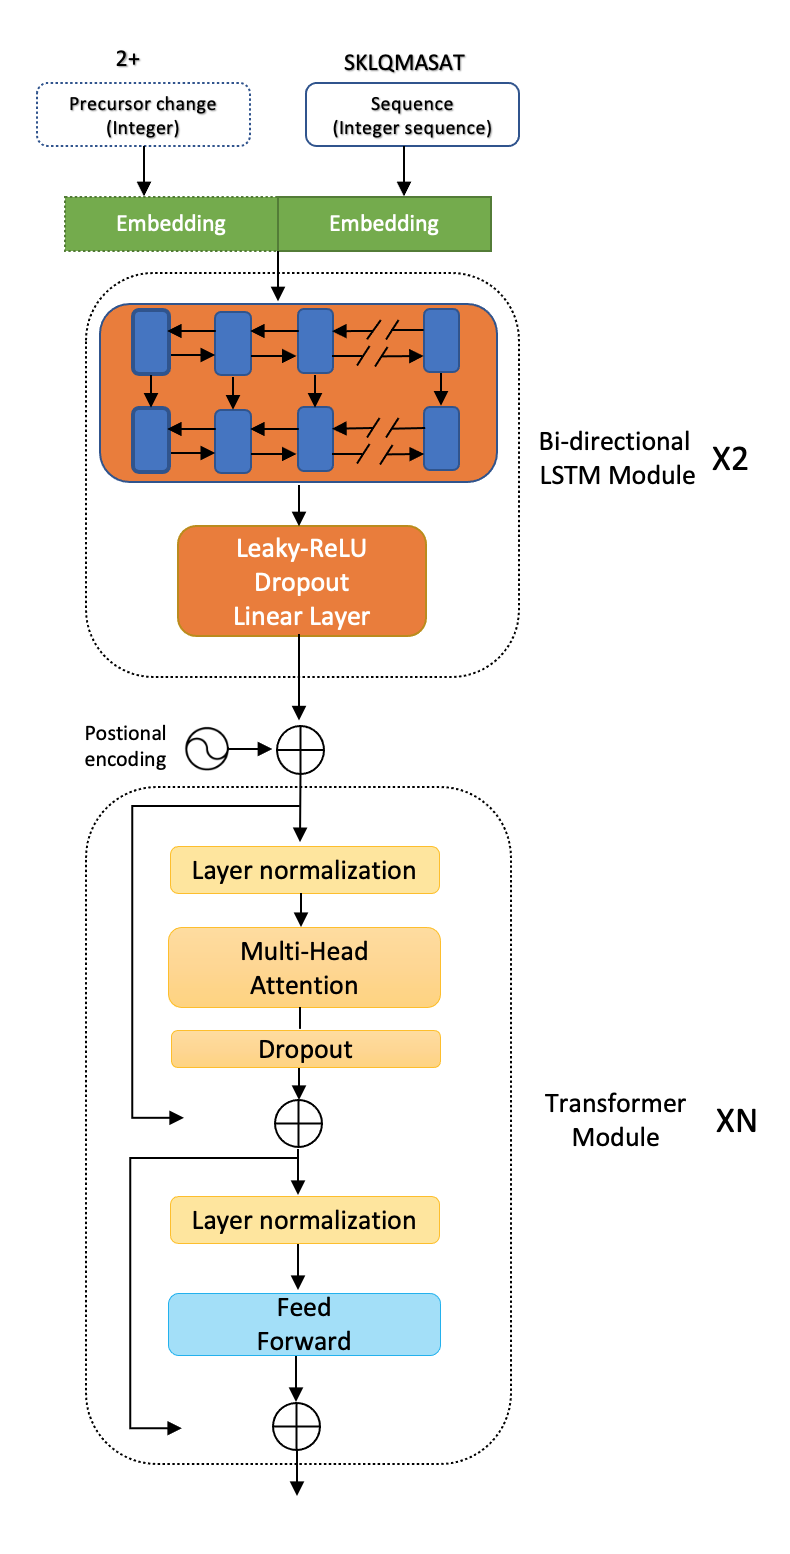
\includegraphics[width=3.0in]{arch}

   \caption{Illustration of model architecture.}
\label{fig:long}
\label{fig:onecol}
\end{figure}

%------------------------------------------------------------------------
\section{Methods}

\subsection{Model method interpretation}

It could be formulated as a regression problem from sequence to value: given sequence \( X \), a learned 
function \( F \) could map the \( X \) to the \( y \), either retention time or ion intensity. The mathematical expression is as follows: 

\[ \hat{y} = F(X;\Theta) \]
$\Theta$ is the parameters of the model.

we find the optimal parameters \( \Theta^\star\) by minimize the loss function \( L \).
\[ \Theta^\star = \arg\min_{\Theta} L(\hat{y},  y) \]


We use the LSTM + Transformer model (illustrated in the Figure~\ref{fig:onecol}) to solve the retention time (RT) and ion intensity prediction task. 
The LSTM module comprises a stack of two units of two layers bi-directional LSTM, and transformer module is composed of 
n layer transformer encoder layer. 

LSTM is a kind of recurrent neural network(RNN) trying to use gate function to capture the long dependency in the input sequence. 
For sequential patterns at position t with input x t and output $y_t$ , $y_t$ does not only rely on $x_t$ but also relies on the 
internal states of previous patterns. LSTM can remember the states of sequential patterns from position 0 to position t − 1 
in the hidden neurons and then predict $y_t$ by combining $x_t$ and the current states of the sequential patterns.
The bi-directional LSTM, expecting to learn a good token embedding for the network's downstream layers, is scheduled as the first module
of our model. Transformer\cite{vaswani2017attention} is the second module, an entirely different model by exploiting the self-attention compared to RNN. 
Self-attention, sometimes called intra-attention is an attention mechanism relating different positions of a single sequence in 
order to compute a representation of the sequence. Self-attention has been used successfully in a variety of tasks including reading 
comprehension, abstractive summarization, textual entailment and learning task-independent sentence representations.
Transformer is the first transduction model relying entirely on self-attention to compute representations of its input and output without 
using sequence aligned RNNs or convolution.
and it has achieved state-of-the-art performance in multiple natural language tasks, such as language translation, language 
entailment classification, language modeling, etc. We use the pre-layer form of transformer, which is proposed in \cite{xiong2020layer}.
The original transfer which locates the layer normalization outside the residual blocks, 
the expected gradients of the parameters near the output layer are large at the beginning of the optimization.
This leads to an unstable training when using a large learning rate. The pre-layernorm version of Transformer which 
 locates the layer normalization inside the residual blocks, can be trained without the warm-up stage and converges much faster.

%-------------------------------------------------------------------------
\subsection{RT prediction}

For this task, we implement 
models with 2 transformer encoder layer.
Especially, since the output of transformer is the same length as the input sequence, we need to take it down to one scaler for 
retention time. By adding the time distributed linear layer to assign varied weights for different amino acids dynamically,
we use the weighted sum to obtain the final prediction. 

Herein we use root of mean squared error (RMSE) as loss function \( L_{RT} \).
\[ L_{RT} = \sqrt{\frac{1}{N}\sum_{i}^N\|\hat{y_{i}} - y_{i}\|^2} \]
Pearson Correlation Coefficient (PCC) is used as metric, implemented in scipy.stats.pearsonr 
\url{www.scipy.org} and defined as:
\[ PCC = \frac{\sum{(x-m_{x})(y-m_{y})}}{\sqrt{\sum{(x-m_{x})^2\sum{(y-m_{y})^2}}}}\]
$m_{x}$ is mean of vector x, and $m_{y}$ is mean of vector y.
The $\Delta$$t_{95\%}$ metric is also used, which represents 
the minimal time window containing the deviations between observed and predicted RTs for 95\% of 
the peptides. 
\[ \Delta t_{95\%} = 2 * | y - \hat{y} |_{95\%} \]

%-------------------------------------------------------------------------
\subsection{Ion intensity prediction}

For ion intensity prediction, we only use one model whose number of transformer encoder layer is 8. Since the output length is 
the same with the sequence, we do not configure a time distributed linear layer.
The model predicts four types of b ion and y ion for this task: ion charged one or two, combined with neural loss or one phosphate loss,
so that we predict eight kinds of ions in total. 

We use mean squared 
error (MSE) as our loss function \( L_{ion} \).
\[ L_{ion} = \frac{1}{N}\sum_{i}^N\|\hat{y_{i}} - y_{i}\|^2 \]
We compute each peptide's PCC and select the median of those PCCs as the final evaluation metric, 
Primarily, we follow Prosit\cite{gessulat2019prosit} using normalized 
spectral angle(SA) as another metric. Similarly, the median of those SAs is reported as the final evaluation metric.
For both RT and Ion intensity tasks, we use Adam optimizer.  
\[ SA = 1 - 2 * \frac{cos^{-1}(\hat{V_a}\cdot\hat{V_b})}{\pi} \]
$\hat{V}$ is a vector whose L2 norm equals 1.
%-------------------------------------------------------------------------
\section{Experiments}
\subsection{RT experiments}
For this task, we compare results of two datasets of our model with DeepRT and different model architecture setting, the performance
is shown in table \ref{table:Human}, Figure \ref{fig:Human_results} and table \ref{table:Jeff}, Figure \ref{fig:Jeff_results}. We could see that we use the 
half number of parameters of DeepRT but achieve better performance in two datasets. And our model's prediction could
fit the real RT distribution very well.

\begin{figure}[t]

   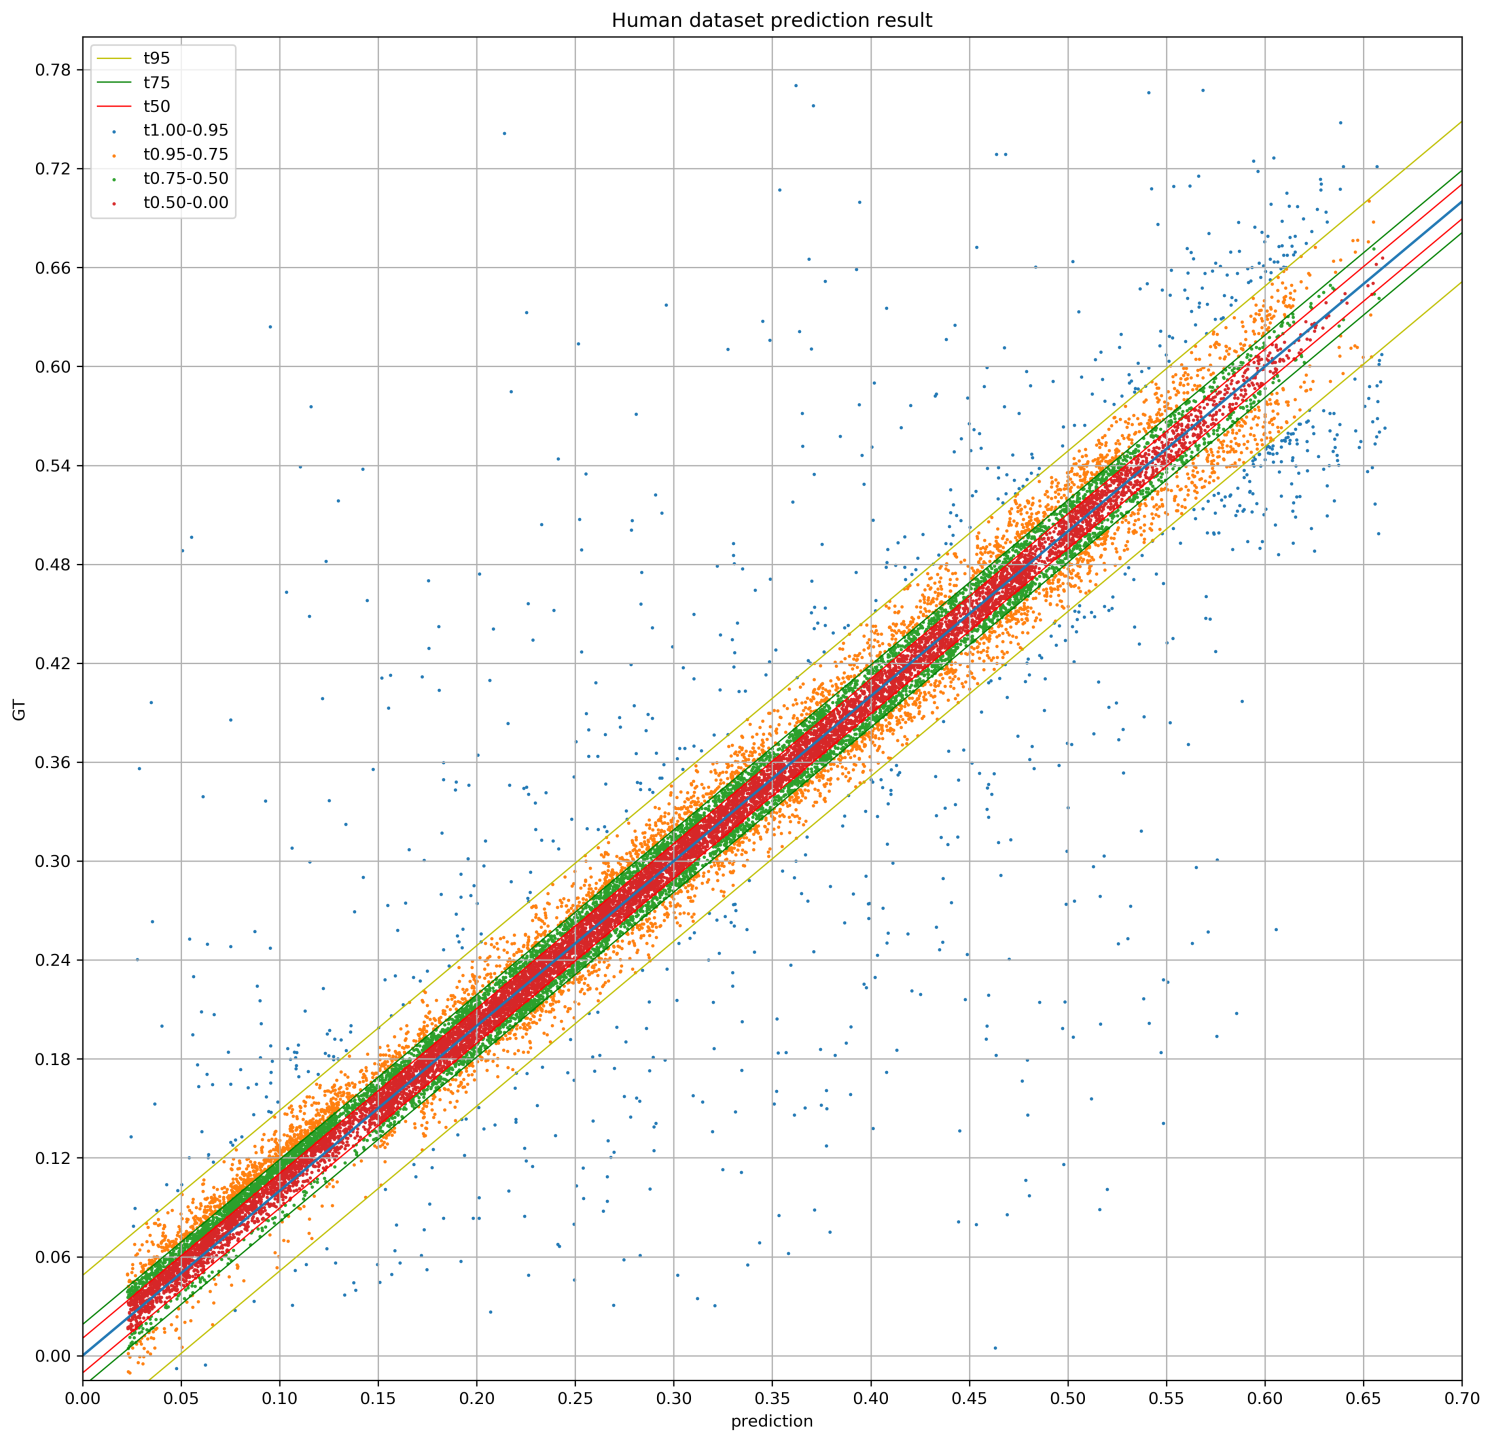
\includegraphics[width=3.0in]{Human_results}

   \caption{Visualization of human dataset}
% \label{fig:long}
\label{fig:Human_results}
\end{figure}

\begin{figure}[t]

   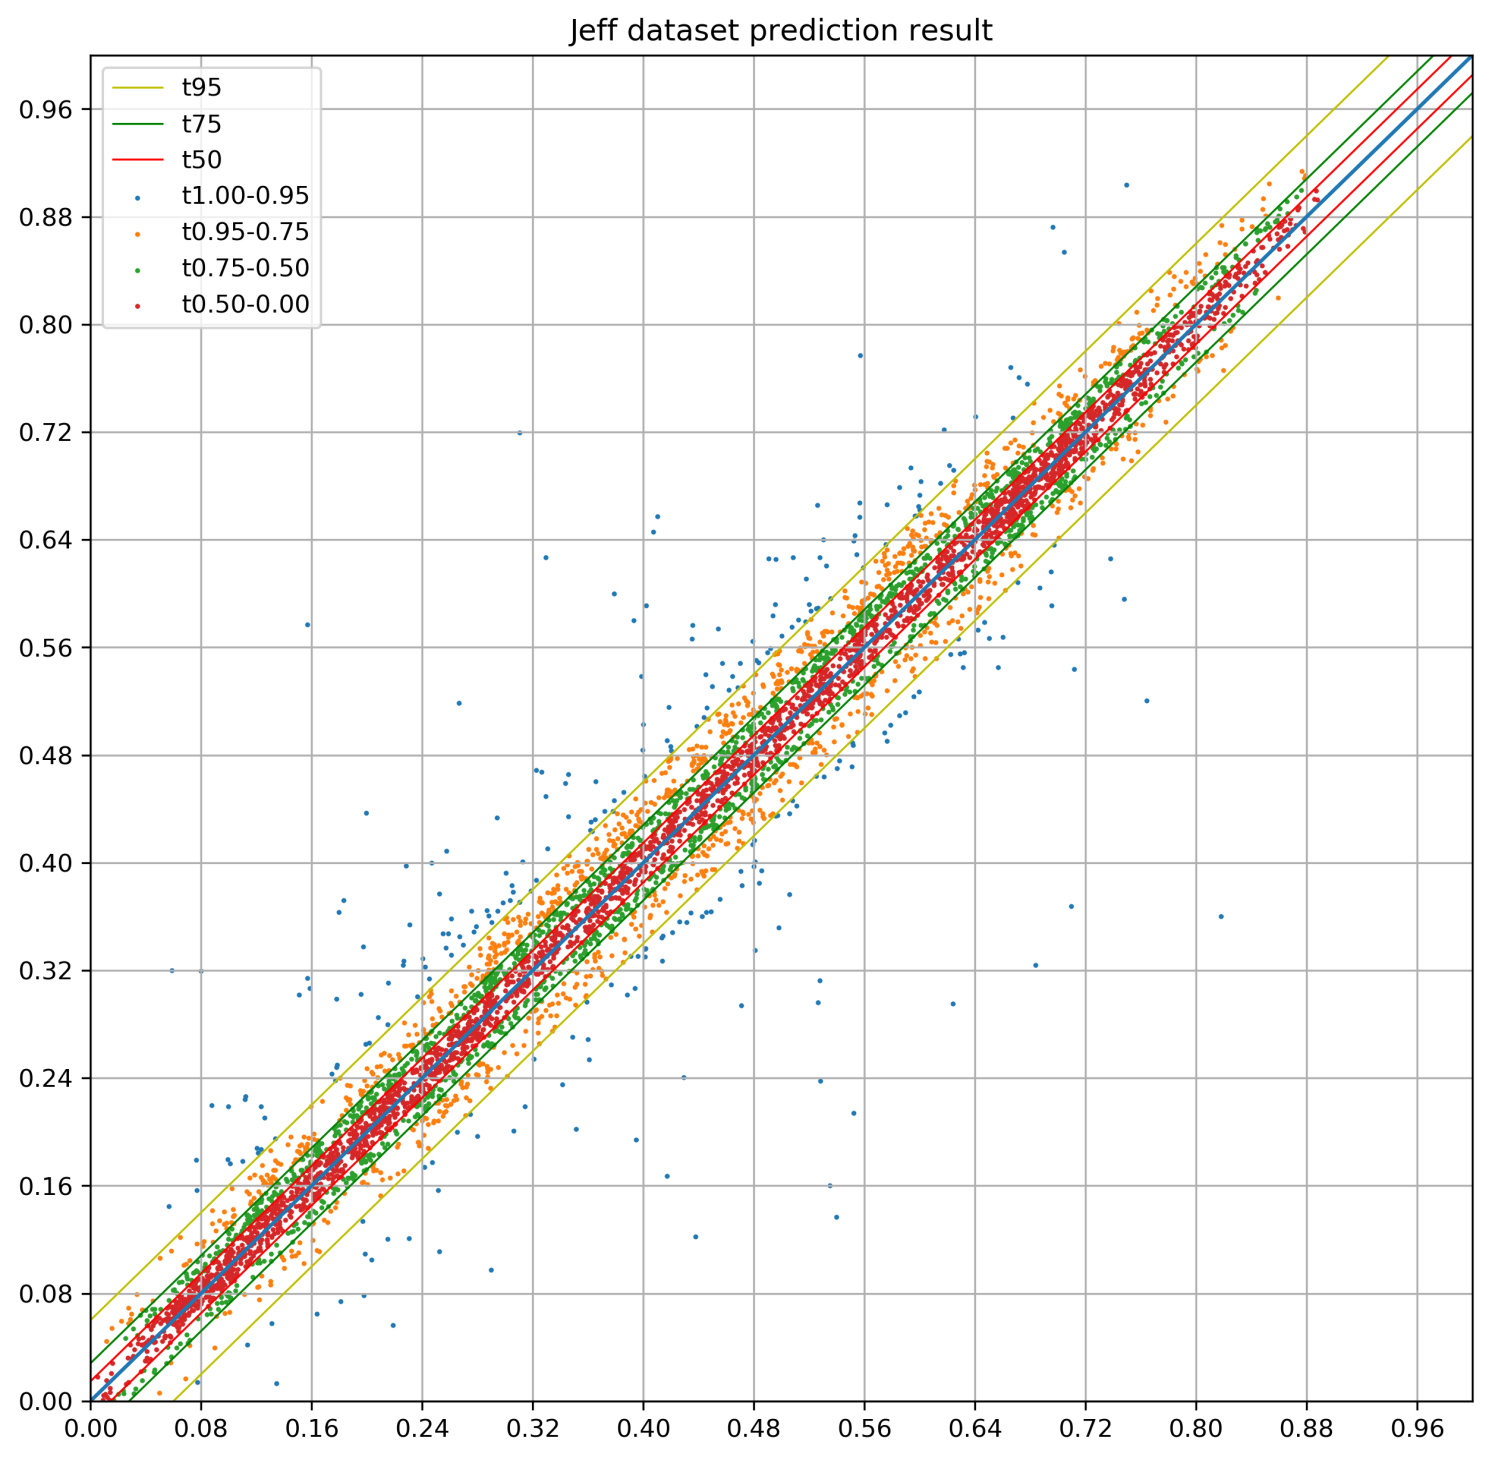
\includegraphics[width=3.0in]{Jeff_results}

   \caption{Visualization of Jeff dataset}
\label{fig:Jeff_results}
\end{figure}

\subsection{Ion Intensity experiments}
As we have explore the architecture in the RT task, so that we only compare with the pdeep2.
The DDA comparison is shown in Figure \ref{fig:DDA}, Table \ref{table:DDA} and Figure \ref{fig:DIA18},
Table \ref{table:DIA18}.
From the results, we could see that in the metric median PCC and SA, we have beaten the SOTA model
pdeep2. In further, to explain our model's good generalization ability, we train our model in the DDA 
dataset and direct test on the DIA18 dataset. Results are show in the Figure \ref{fig:DIA18_direct} and Table \ref{table:DIA18_direct}.
And we could see results that model trained on the DDA dataset, test on DIA18 dataset are comparable to trained
on DIA18, and are even similar to pdeep2's results on DIA18.
%-------------------------------------------------------------------------

\begin{figure}[t]

   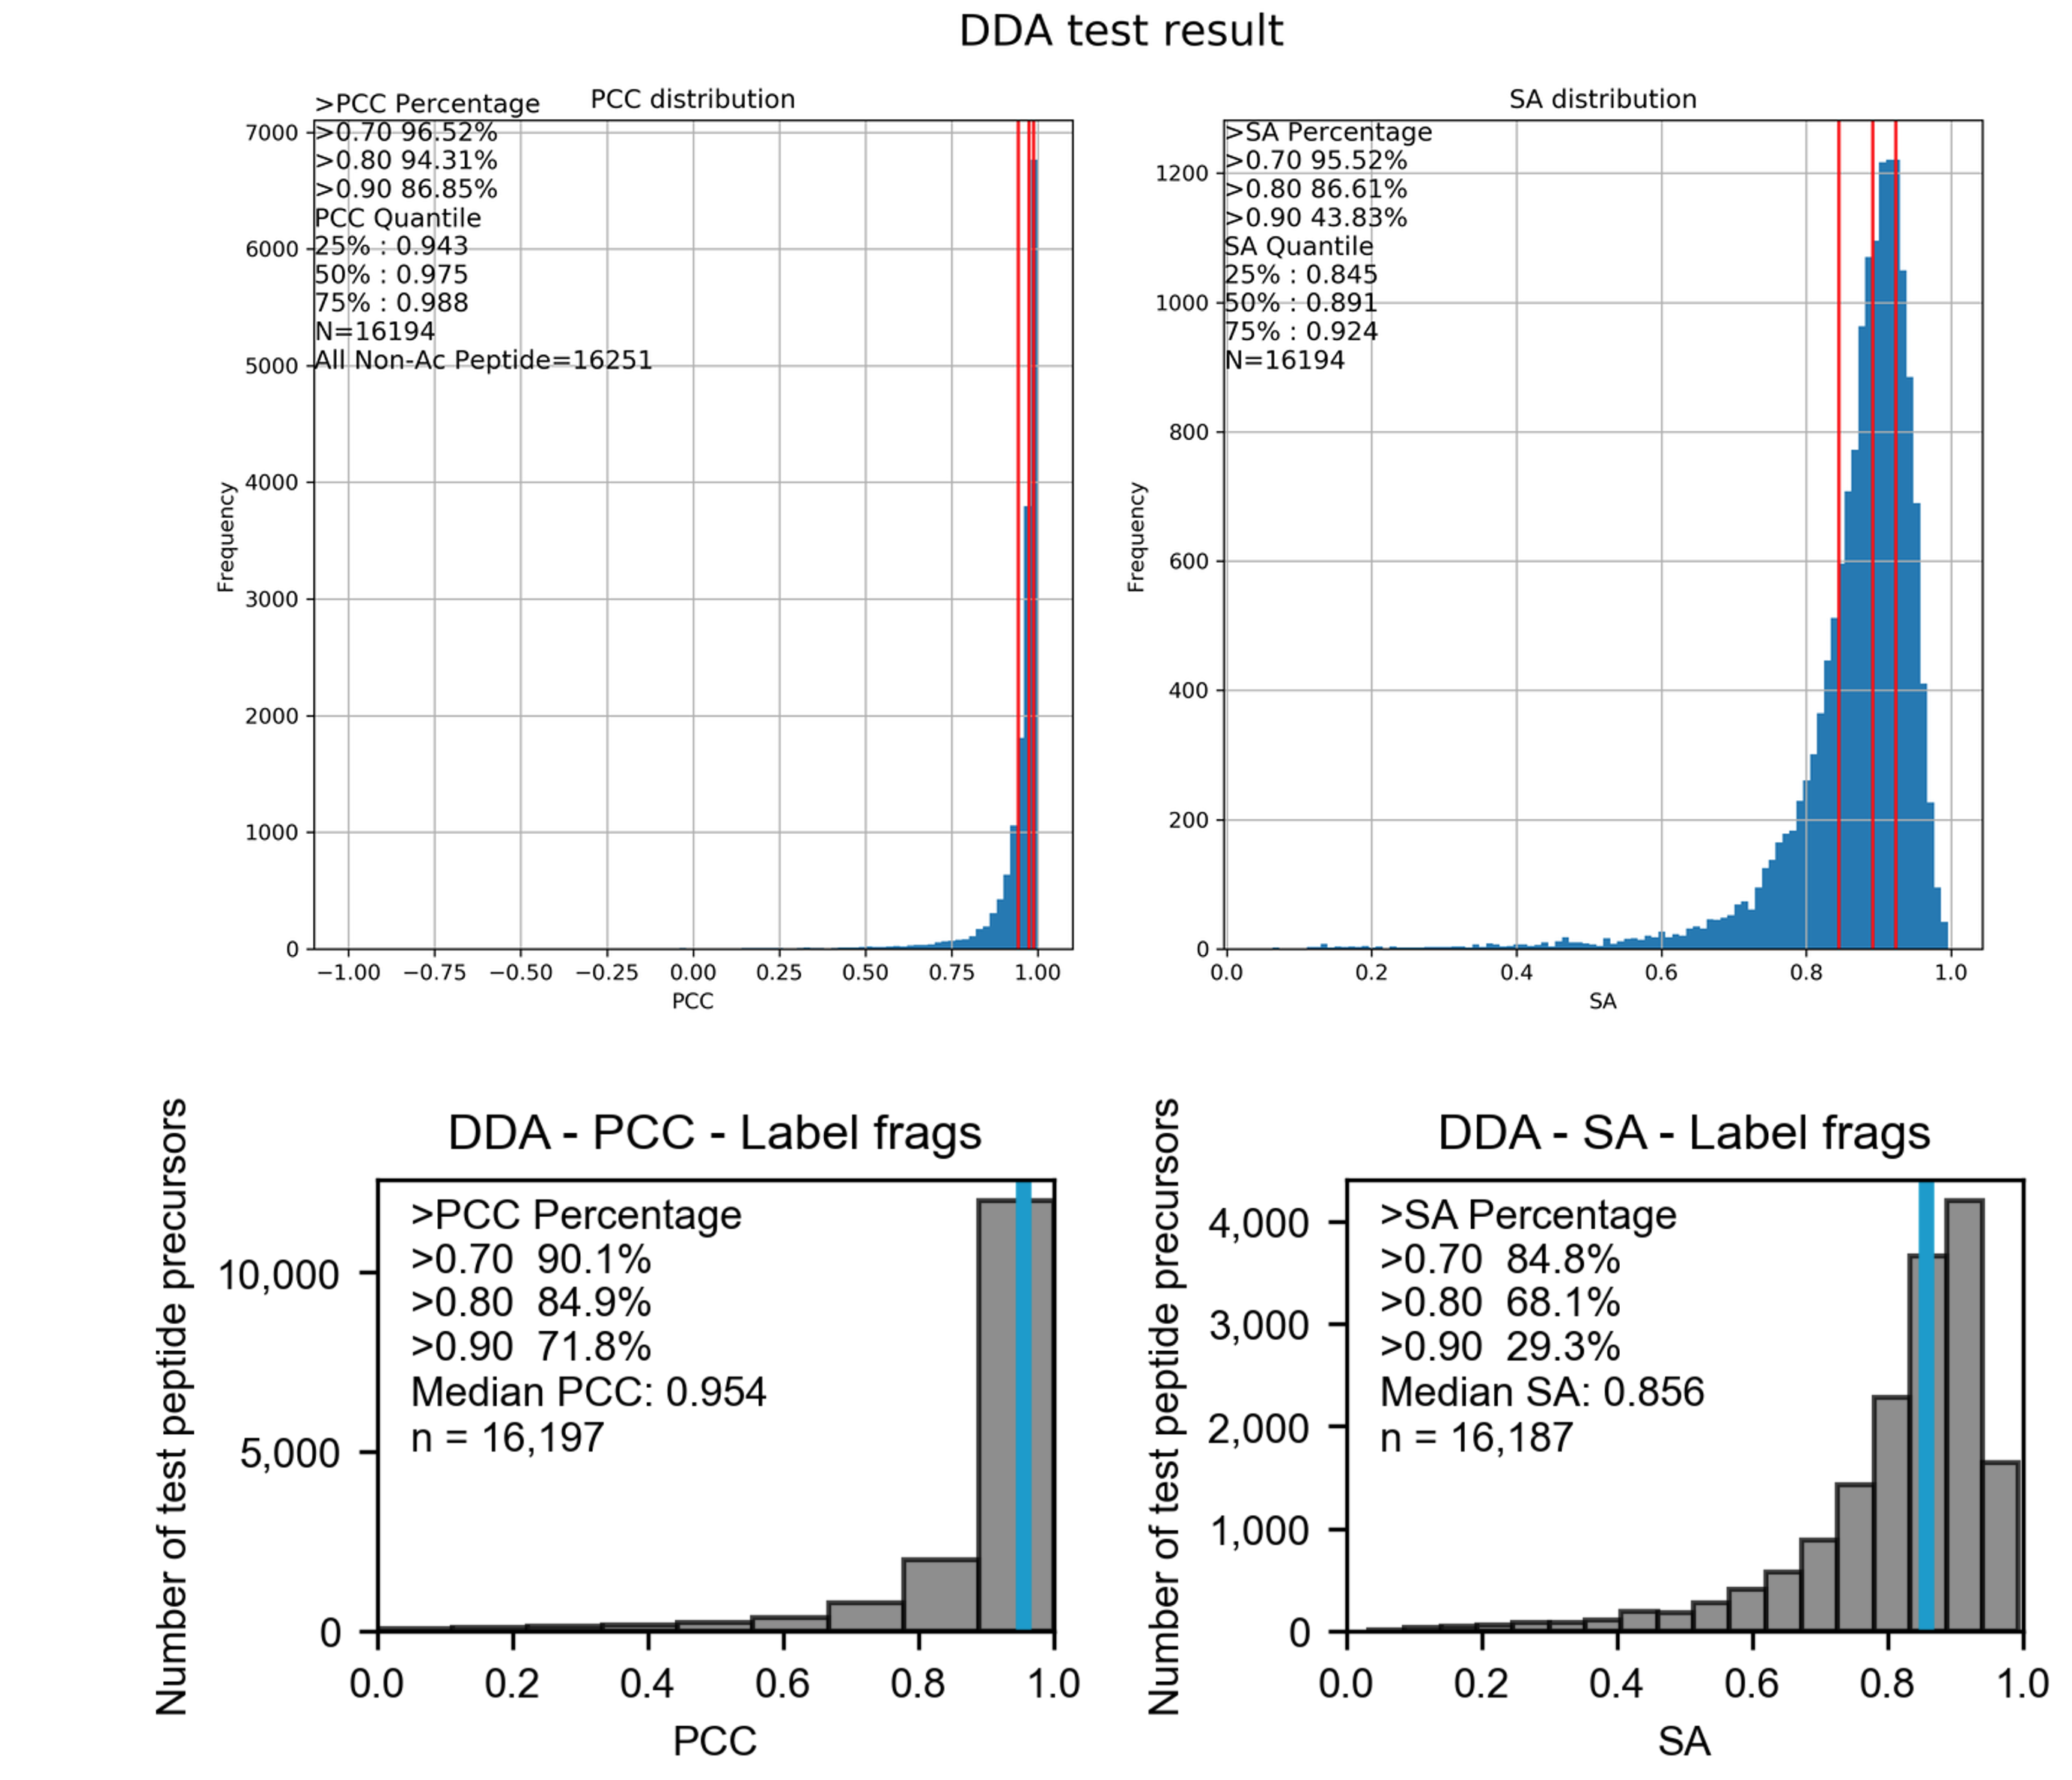
\includegraphics[width=3.0in]{DDA}

   \caption{Visualization of performance of DDA dataset. The above is ours and the below is pdeep2}
\label{fig:DDA}
\end{figure}


\begin{figure}[t]

   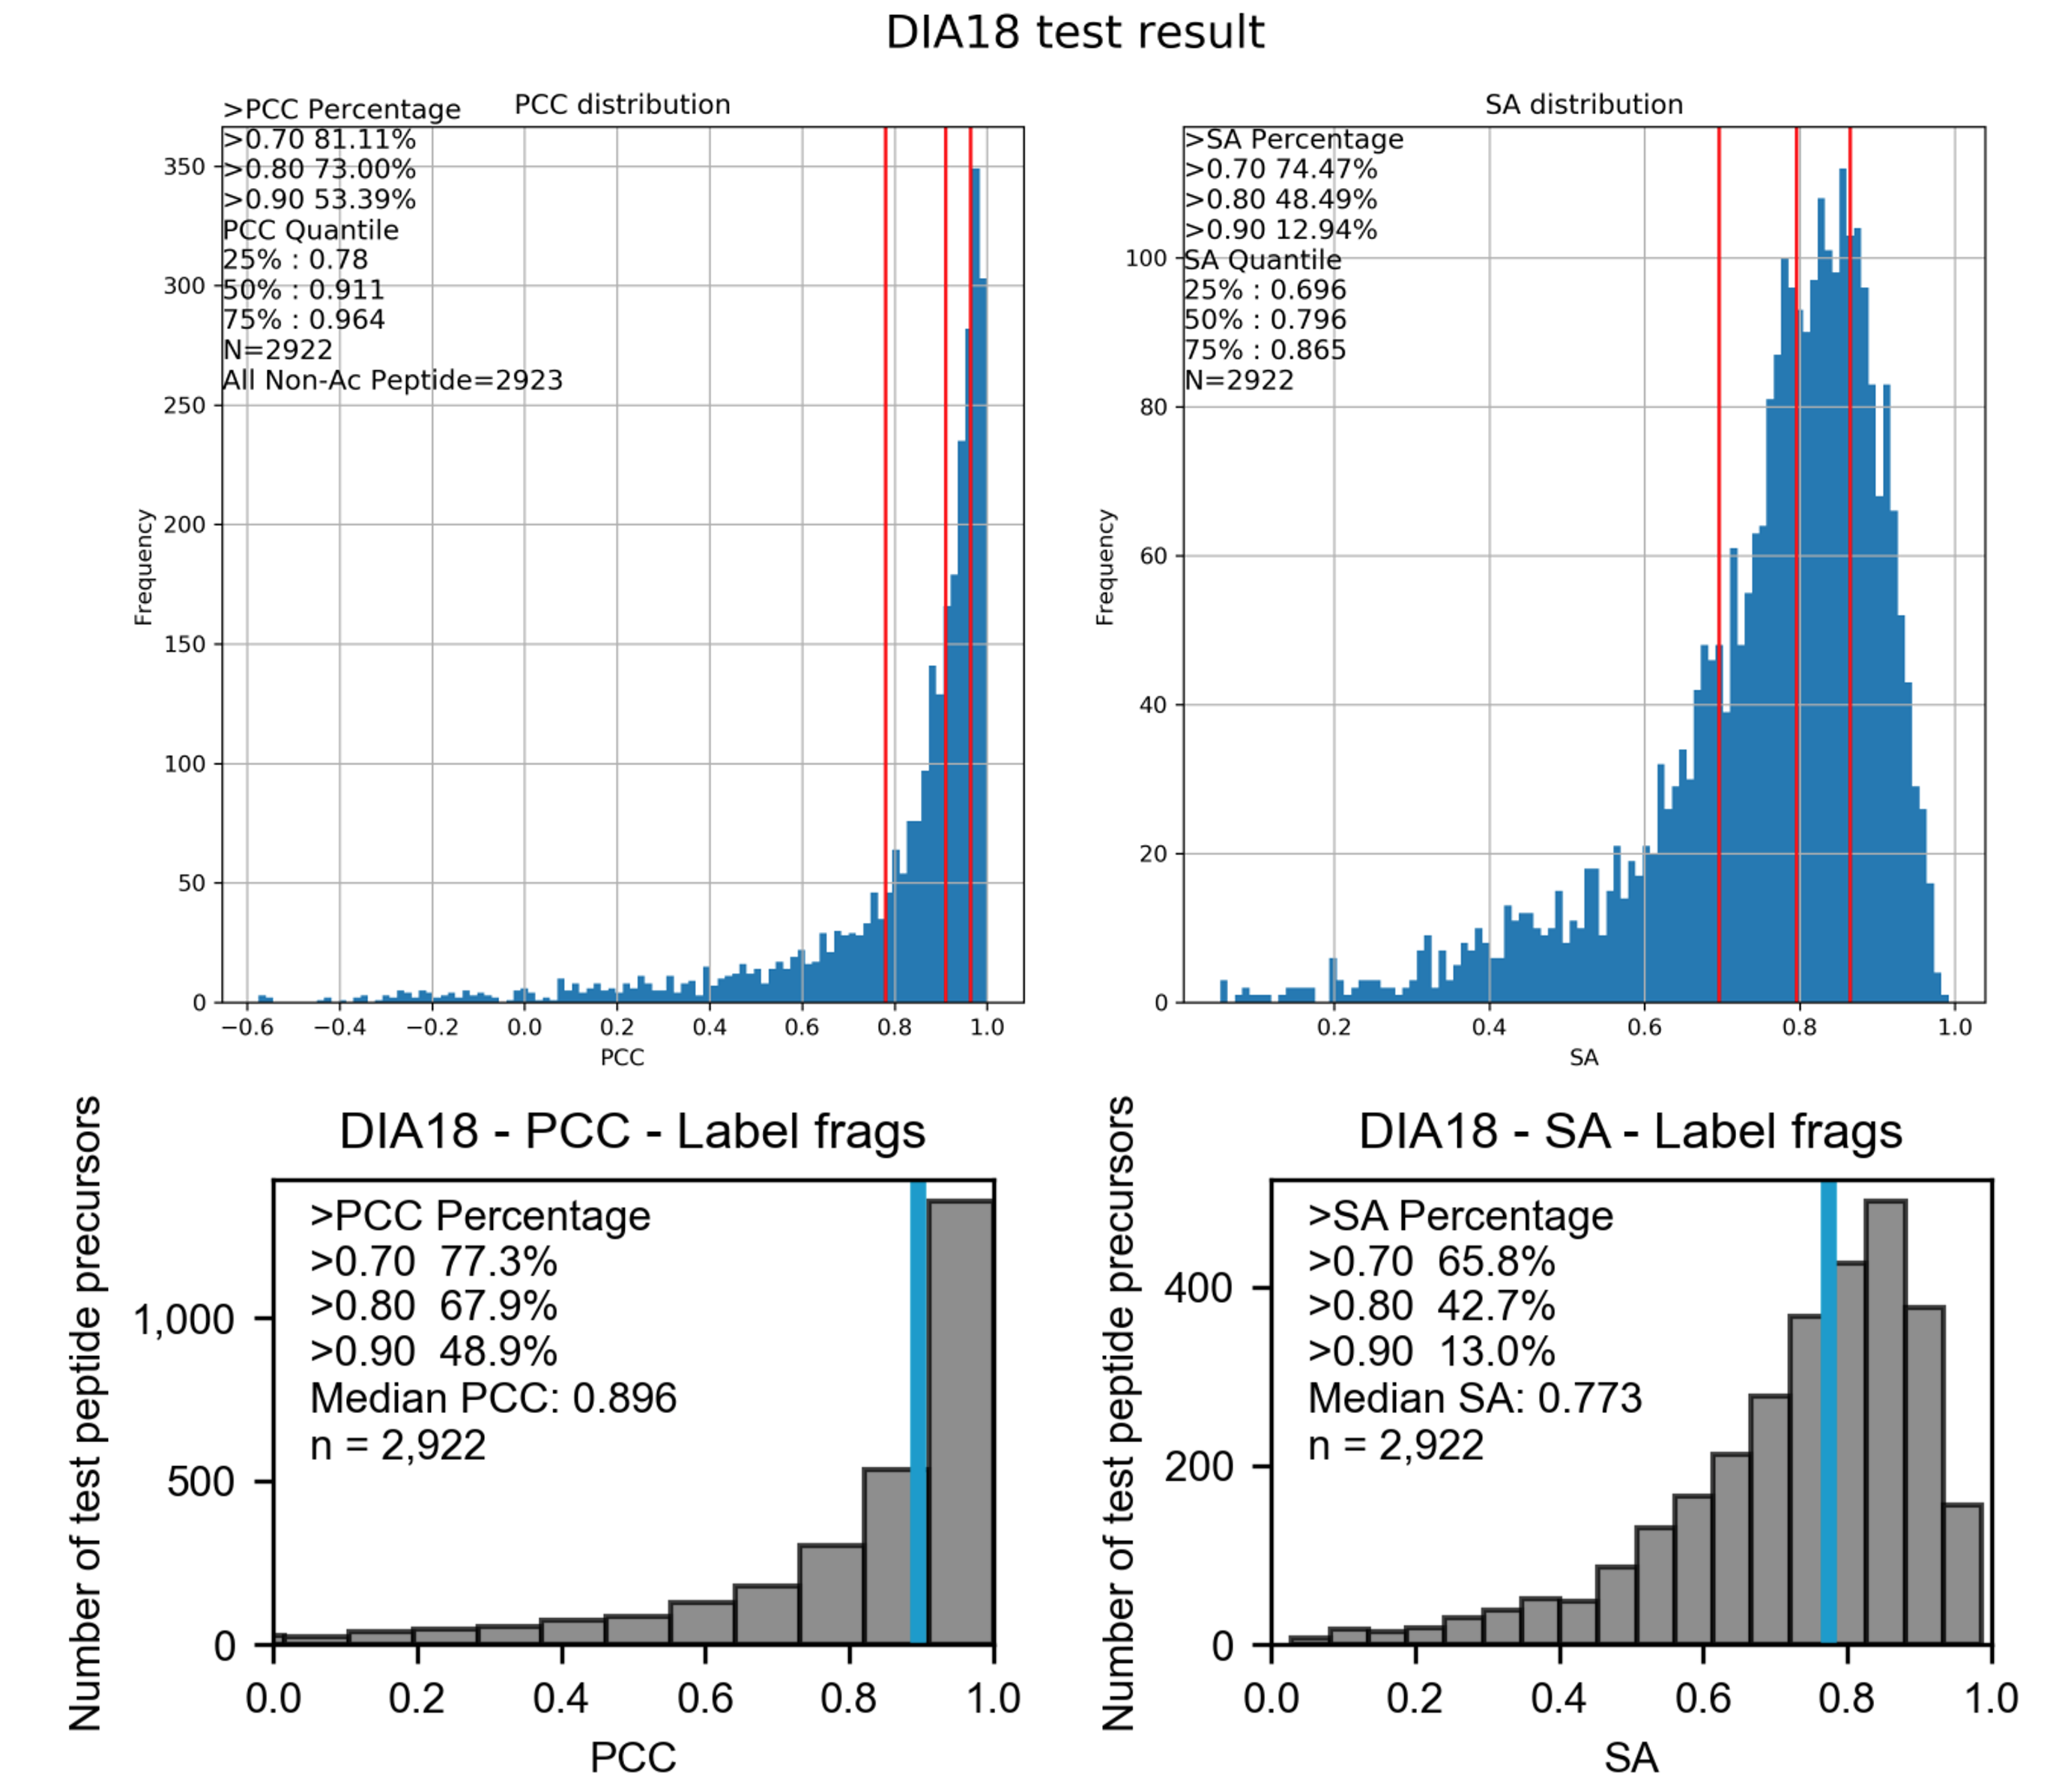
\includegraphics[width=3.0in]{DIA18}

   \caption{Visualization of DIA18 dataset.  The above is ours and the below is pdeep2}
\label{fig:DIA18}
\end{figure}


\begin{figure}[t]

   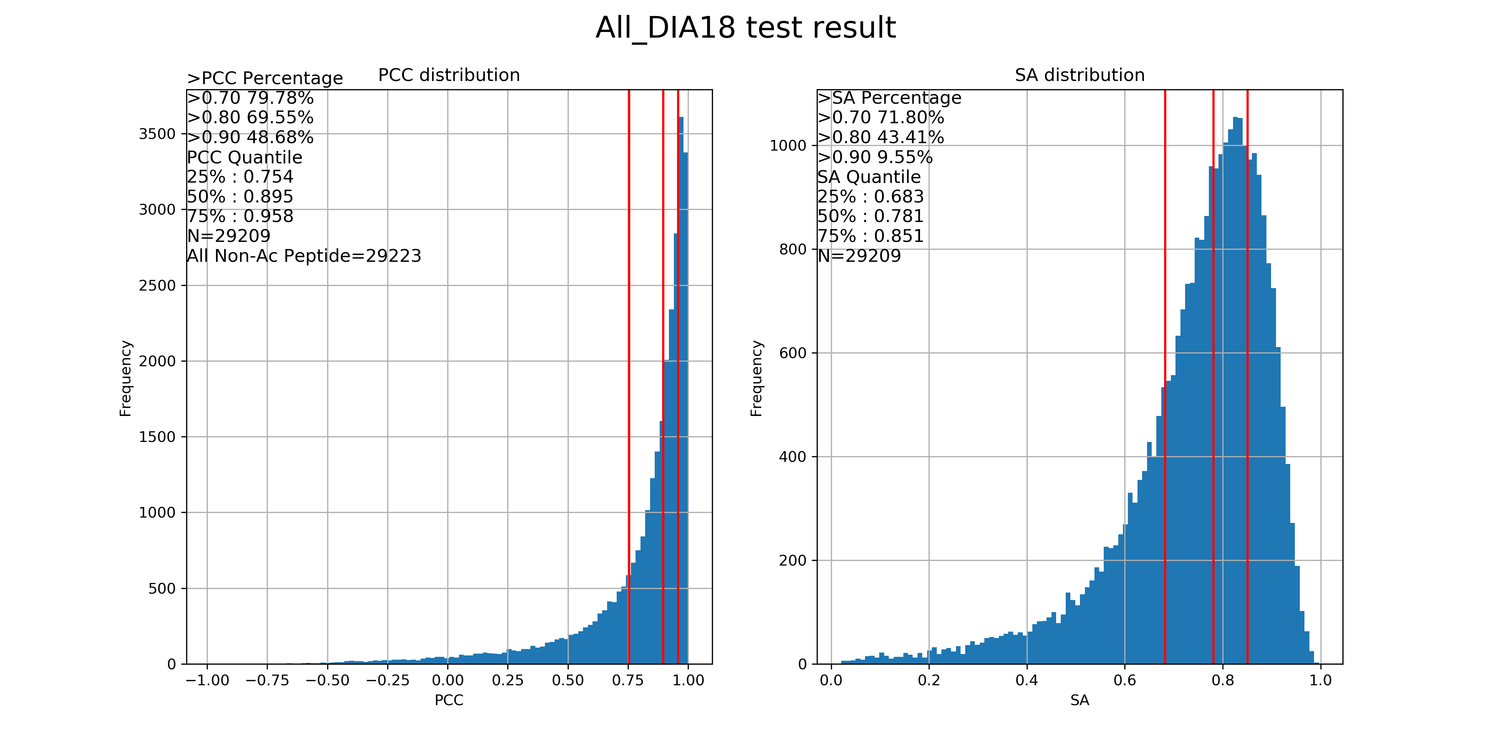
\includegraphics[width=3.5in]{DIA_direct_test}

   \caption{Direct test on DIA18 dataset.}
\label{fig:DIA18_direct}
\end{figure}

\begin{table}
   \begin{center}
   \begin{tabular}{|l|c|c|}
   \hline
   Model & $\Delta$$t_{95\%}$ & parameters \\
   \hline\hline
   DeepRT & 15.67 & 3.1M \\
   LSTM & 14.73 & 1.1M \\
   LSTM+transformer(ours) & 14.70 & 1.5M \\
   transformer & 17.00 & 3M \\
   \hline
   \end{tabular}
   \end{center}
   \caption{Human Dataset results.   Ours is better.}
   \label{table:Human}
   \end{table}
   
   
   \begin{table}
      \begin{center}
      \begin{tabular}{|l|c|c|}
      \hline
      Model & $\Delta$$t_{95\%}$ & parameters \\
      \hline\hline
      DeepRT & 19.7 & 3.1M \\
      LSTM & 17.6 & 1.1M \\
      LSTM+transformer(ours) & 17.3 & 1.5M \\
      transformer & 20.8 & 3M \\
      \hline
      \end{tabular}
      \end{center}
      \caption{Jeff Dataset results.   Ours is better.}
      \label{table:Jeff}
      \end{table}

\begin{table}
   \begin{center}
   \begin{tabular}{|l|c|c|}
   \hline
   Model & Median PCC & Median SA \\
   \hline\hline
   pdeep2 & 0.954 & 0.856 \\
   LSTM+transformer$\star$ & 0.975 & 0.891 \\
   \hline
   \end{tabular}
   \end{center}
   \caption{DDA Dataset results.Ours is better.}
   \label{table:DDA}
   \end{table}

\begin{table}
   \begin{center}
   \begin{tabular}{|l|c|c|}
   \hline
   Model & Median PCC & Median SA \\
   \hline\hline
   pdeep2 & 0.896 & 0.773 \\
   LSTM+transformer$\star$ & 0.911 & 0.796 \\
   \hline
   \end{tabular}
   \end{center}
   \caption{DIA18 Dataset results.Ours is better.}
   \label{table:DIA18}
\end{table}

\begin{table}
   \begin{center}
   \begin{tabular}{|l|c|c|}
   \hline
   Model & Median PCC & Median SA \\
   \hline\hline
   Direct Test & 0.895 & 0.781 \\
   Train then Test & 0.911 & 0.796 \\
   \hline
   \end{tabular}
   \end{center}
   \caption{DIA18 Dataset results. Direct test only drops little compared to training and test}
   \label{table:DIA18_direct}
\end{table}
%-------------------------------------------------------------------------
\section{Conclusion}

In this study, we introduce Dive2Protein, a flexible deep neural network architecture able to predict retention times and 
tandem mass spectrometry spectra of peptides and that substantially surpass current 
benchmarks and tools. Although trained on tryptic peptides from human origin, it performed very well with all proteases, 
organisms, datasets, mass spectrometers and acquisition parameters tested here. This highlights that the learned internal 
representation of Dive2Protein approximates a chemo-physical model for peptide fragmentation and chromatographic retention time. 
However, it is also clear that including more non-tryptic data or longer peptides as well as higher charge states would 
most probably further improve prediction accuracy.

Our collaborator's results demonstrate that predicted spectral libraries can be used for analyzing DIA data. While predicted 
libraries performed slightly worse than high-quality experimental spectral libraries, replacing lower quality 
spectral libraries by consistent and high signal-to-noise predicted spectra increased the number of identified 
peptides by up to 10$\%$. In the future, Dive2Protein might enable the regeneration of libraries on instrument replacement 
or calibration and potentially supports the consistent addition of new peptide hypothesis without compromising 
the homogeneity of a library.




{\small
\bibliographystyle{ieee_fullname}
\bibliography{egbib}
}

\end{document}
